% %%%%%%%%%%%%%%%%%%%%%%%%%%%%%%%%%%%%%%%%%%%%%%%%%%%%%%%%%%%
% Hier nichts aendern
\documentclass[sigconf, nonacm, review]{acmart}
\AtBeginDocument{%
  \providecommand\BibTeX{{%
    \normalfont B\kern-0.5em{\scshape i\kern-0.25em b}\kern-0.8em\TeX}}}

\setcopyright{acmcopyright}
\copyrightyear{2018}
\acmYear{2018}
\acmDOI{XXXXXXX.XXXXXXX}
\acmJournal{JACM}
\acmVolume{37}
\acmNumber{4}
\acmArticle{111}
\acmMonth{8}
\acmPrice{15.00}
\acmISBN{978-1-4503-XXXX-X/18/06}
% Hier nichts aendern
% %%%%%%%%%%%%%%%%%%%%%%%%%%%%%%%%%%%%%%%%%%%%%%%%%%%%%%%%%%%

\begin{document}
% %%%%%%%%%%%%%%%%%%%%%%%%%%%%%%%%%%%%%%%%%%%%%%%%%%%%%%%%%%%
% Hier eigene Daten eingeben
\title{Report zum Fachprojekt Routingalgorithmen}
\author{Pouria Araghchi}
\affiliation{%
  \institution{TU Dortmund}
  \streetaddress{Otto-Hahn-Stra\ss e 14}
  \city{Dortmund}
  \country{Deutschland}}
\email{pouria.araghchi@tu-dortmund.de}

\author{Kai Lukas Ilmenau}
\affiliation{%
  \institution{TU Dortmund}
  \streetaddress{Otto-Hahn-Stra\ss e 14}
  \city{Dortmund}
  \country{Deutschland}}
\email{kai.ilmenau@tu-dortmund.de}

\author{Naveed Niazi}
\affiliation{%
  \institution{TU Dortmund}
  \streetaddress{Otto-Hahn-Stra\ss e 14}
  \city{Dortmund}
  \country{Deutschland}}
\email{naveed.niazi@tu-dortmund.de}

\renewcommand{\shortauthors}{Araghchi, Ilmenau, Niazi}
% Hier eigene Daten eingeben
% %%%%%%%%%%%%%%%%%%%%%%%%%%%%%%%%%%%%%%%%%%%%%%%%%%%%%%%%%%%

\begin{abstract}
In diesem Report werden die Ergebnisse unserer Arbeit im Rahmen des Fachprojekts "Routingalgorithmen" zusammengefasst.
Wir haben die Algorithmen auf die \emph{Maximum Link Utilization} (MLU) nach \cite{foerster2021} untersucht.
In einem der drei F\"alle wurde die sequentielle Kombination aus dem $inverse\_capacity$-Algorithmus und dem $demand\_first\_waypoints$-Algorithmus untersucht.
Der Algorithmus, der \emph{inverse capacity} mit centrality Metriken verrechnet, ist meistens schlechter als \emph{inverse capacity}, 
da reines \emph{inverse capacity} \"ofter zwei k\"urzeste Wege findt um demands gleichm\"a\ss iger zu verteilen und damit einzelne Links nicht \"uberlastet werden.
Es wird jedoch auch gezeigt, dass Topologien gefunden werden k\"onnen, bei den pures \emph{inverse capacity} eine schlechtere MLU hat.
Ein weiterer Algorithmus befasst sich mit der sequenziellen Kombination von Open Shortest Path First (OSPF) mit zwei verschiedenen Algorithmen: 
Demand First Waypoint (DFW) und Uniform Weights (UW).
Die Replikation einer anderen Gruppe im ersten Projektteil nicht erfolgreich, und im zweiten schon, 
jedoch haben wir daraus die Lehre gezogen wie wir unsere Arbeit besser replizierbar machen und das fr\"uhe Kommunikation mit den anderen Gruppen wichtig ist.
\end{abstract}

\begin{CCSXML}
<ccs2012>
<concept>
<concept_id>10003033.10003068.10003073.10003076</concept_id>
<concept_desc>Networks~Traffic engineering algorithms</concept_desc>
<concept_significance>500</concept_significance>
</concept>
</ccs2012>
\end{CCSXML}

\ccsdesc[500]{Networks~Traffic engineering algorithms}

% Eventuell keywords weglassen
\keywords{weight optimization, waypoint optimization}

\received{6. August 2023}
\received[\"uberarbeitet]{9. August 2023}
\received[akzeptiert]{15. August 2023}

\maketitle

% %%%%%%%%%%%%%%%%%%%%%%%%%%%%%%%%%%%%%%%%%%%%%%%%%%%%%%%%%%%%%%%%%%
% Einleitung
% %%%%%%%%%%%%%%%%%%%%%%%%%%%%%%%%%%%%%%%%%%%%%%%%%%%%%%%%%%%%%%%%%%
\section{Einleitung}
In der heutigen Zeit werden mehrere Millionen Datenpakete von und zu Knotenpunkten verschickt.
Daher ist das \emph{Routing} von diesen Datenpaketen in der heutigen Zeit wichtiger denn je.
Gutes Routing kann Datenstaus verringern oder sogar verhindern, Verteilerknoten auslasten oder entlasten 
und sorgt damit f\"ur einen reibungslosen Datenverkehr \"uberall auf der Welt.
Wie gut das Routing innerhalb einer Netzwerktopologie ist, 
wird durch den darunterliegenden Routingalgorithmus bestimmt.
Hierf\"ur gibt es verschiedenste Ans\"atze mit variierender Komplexit\"at und Erfolgswahrscheinlichkeit.

Im Rahmen des Fachprojekts "Routingalgorithmen" haben wir uns n\"aher mit den verschiedenen Algorithmen besch\"aftigt 
und haben eigene Variationen dieser Algorithmen erstellt,
um ein tieferes Verst\"andnis der Materie zu erlangen.
Zielfunktion war hierbei die \emph{Maximum Link Utilization} (MLU) nach \cite{foerster2021}.
In diesem Report fassen wir die Ergebnisse unserer Arbeit zusammen.
Dies umfasst eine Beschreibung unserer drei algorithmischen Ideen (Sequential combination aus \emph{inverse capacity} und demand
first waypoints, centrality Metriken mit \emph{inverse capacity} und Sequential combination aus \emph{inverse capacity} und \emph{demand first waypoints})
und Experimente zu Algorithmen im Stil des Papers\cite{foerster2021}.
Danach werden die Resultate dieser Experimente eingeordnet und erkl\"art.
Anschließend wird auf die Arbeit einer anderen Gruppe im Fachprojekt eingegangen, deren Arbeit wir im Rahmen dieses Fachprojekts repliziert haben.


% %%%%%%%%%%%%%%%%%%%%%%%%%%%%%%%%%%%%%%%%%%%%%%%%%%%%%%%%%%%%%%%%%%
% Theorie
% %%%%%%%%%%%%%%%%%%%%%%%%%%%%%%%%%%%%%%%%%%%%%%%%%%%%%%%%%%%%%%%%%%
\section{Theoretische Grundlagen}
Die Grundlage zu dieser Arbeit bildet das Paper "Traffic Engineering with Joint Link Weight and Segment Optimization"\cite{foerster2021}.
In der Artbeit wurdeb alternativen Routing-Algorithmen gesucht, 
welche eine optimale \emph{minimal link utilization} (MLU) auf diversen Topologien -- synthetische sowie reale -- liefern. 
Zwei Algorithem und insbesondere deren Verkn\"upfung haben sich als vorteilhaft erwiesen.
\subsubsection{Link-Weight-Optimization} 
Im Allgemeinen werden f\"ur den Datenpakettransfer k\"urzeste Pfade ermittelt.
Hierf\"ur werden die Kanten, die die Knoten innerhalb einer Topologie verbinden, 
mit Gewichten versehen, 
die als Quantifizierung f\"ur die Distanz oder Attraktivit\"at der jeweiligen Kanten verwendet werden.
Bei der \emph{Link-Weight-Optimisierung} (LWO) geht es darum, 
die Gewichte der Kanten so zu optimieren, 
dass w\"ahrend des Datenflusses Datenstaus vermieden oder vorteilhaft aufgeteilt werden. 
Um das zu erreichen, 
muss die gesamte Topologie betrachtet und desses Gewichte nochmal berechnet werden.
Da das Berechnen optimaler Kanten-gewichte ein NP-hartes Problem ist,
werden in der Regel heuristische Methoden zur Berechnung der Kanten verwendet.
Eine bekannte und weitl\"aufig genutzte ist die $inverse\_capacity$-Methode.
\subsubsection{Waypoint-Optimization}
Wie in dem dieser Arbeits zur grundeliegenden Paper\cite{foerster2021} beschrieben,
reicht es in der Regel nicht aus, einfach nur die Kantengewichte einzustellen, um den anfallenden Datenstau zu verhindern.
Hierf\"ur bietet sich das Setzen von Wegpunkten (englisch: \emph{waypoints}) an, 
da hier der gesamte Datenfluss innerhalb der Topologie ganzheitlich betrachtet wird 
und die Wegpunkte f\"r die jeweiligen Datenfl\"usse so gesetzt werden, 
dass mehrere dieser Fl\"usse nicht entlang derselben Pfade innerhalb der Topologie gef\"uhrt werden, 
wenn die Wegpunkte nicht die n\"tigen Kapazit\"aten haben, um die Daten aller einflie\ss enden Str\"ome ohne Datenstau aufzunehmen und weiterzuleiten.
\subsubsection{Joint Weights and Waypoint Optimization}
Die Kombination aus beiden vorherigen Ans\"atzen ist daraus gewachsen, 
die Schw\"a-chen der einzelnen Methodiken zu auszugleichen.
Dabei eignet sich die LWO im Allgemeinen schlecht, 
um die Kantengewichte der einzelenen Datenfl\"usse getrennt von allen anderen Datenfl\"ussen zu optimieren.
Sobald die Kantengewichte gesetzt wurden, gelten diese f\"ur alle Kanten und f\"ur alle Datenpakete, 
die von einer Quelle zu einem anderen Ziel unterwegs sind.
Dies kann zur Folge haben, dass Gewichte, die f\"ur eine Anforderung gut geeignet sind, weniger optimal f\"ur eine oder mehrere andere Anforderungen sind.
Auf der anderen Seite h\"angt die Effektivit\"at von Wegpunkten (WPO), 
f\"ur sich alleine betrachetet, stark von den zuvor gesetzten Kantengewichten ab.
Daher k\"onnen schlechte beziehungsweise suboptimale Kantengewichte innerhalb einer Topologie zu suboptimalen Wegpunkten f\"ur die Anforderungen der Datenpakete f\"uhren.
Im Rahmen dieses Papers schnitt die Joint-Methode im Vergleich auf verschiedensten Topologien besonders gut ab, 
wie in \cite{foerster2021} gesehen werden kann.
Diese Erkenntnis f\"uhrte zu der Frage, 
wie sich andere Algorithmen oder Methodiken in Verbindung auswirken. 
Mit der Beantwortung dieser Frage befassen sich die folgenden Abschnitte.

% %%%%%%%%%%%%%%%%%%%%%%%%%%%%%%%%%%%%%%%%%%%%%%%%%%%%%%%%%%%%%%%%%%
% Umsetzung
% %%%%%%%%%%%%%%%%%%%%%%%%%%%%%%%%%%%%%%%%%%%%%%%%%%%%%%%%%%%%%%%%%%
\section{Umsetzung}
In diesem Abschnitt werden unsere Projekte und die dazugeh\"origen Ideen vorgestellt.
Die beiden Projekte sind in Unterabschnitte und die algorithmischen Ideen und Umsetzungen des jeweiligen Gruppenmitglieds in Paragraphen unterteilt. 
% %%%%%%%%%%%%%%%%%%%%%%%%%%%%%%%%%%%%%%%%%%%%%%%%%%%%%%%%%%%%%%%%%%
% Projekt 1
% %%%%%%%%%%%%%%%%%%%%%%%%%%%%%%%%%%%%%%%%%%%%%%%%%%%%%%%%%%%%%%%%%%
\subsection{Algorithmen zu Projekt 1}
In Projekt 1 ging es darum, eine algorithmische Idee auf Basis von \cite{foerster2021} herauszuarbeiten und diese mithilfe desselben Git-Projekts\footnote{\url{https://github.com/fruitiestPunch/FaPro_P1}, siehe Abschnitt \ref{sec:resouces}} mit alternativen Routingalgorithmen zu vergleichen. 
% %%%%%%%%%%%%%%%%%%%%%%%%%%%%%%%%%%%%%%%%%%%%%%%%%%%%%%%%%%%%%%%%%%
% Pouria
% %%%%%%%%%%%%%%%%%%%%%%%%%%%%%%%%%%%%%%%%%%%%%%%%%%%%%%%%%%%%%%%%%%
\subsubsection{Sequential combination aus inverse capacity und demand first waypoints}
Der Kerngedanke hier war es, einen einen schnellen Algorithmus zu finden, 
welcher hinreichend gute Ergebnisse in Bezug auf die MLU abliefert.
Diese Eigenschaft ist insbesondere f\"ur Netzwerke sinnvoll,
dessen Auslastungen sich regelm\"a\ss ig w\"ahrend des Betriebs \"andern und der Algorithmus reaktiv sehr schnell alle Gewichte und Wegpunkte neu berechnet.\newline
Die Grundlage dieses Algorithmus war die sequentielle Kombination von dem empirisch h\"aufig verwendetem \emph{inverse capacity} und dem etwas langsameren aber genaueren \emph{demand first waypoints}.
\emph{Anmerkung: Die Algorithemn Namen "\emph{demand first waypoints}" und "\emph{greedy waypoints}" sind hier austauschbar.}\newline
Daraufhin bildeten sich zwei Fragen.
\begin{enumerate}
    \item Ist die Kombination genauer als dessen Bestandsteile?
    \item Ist die zus\"atzliche Rechenzeit gerechtfertigt?
\end{enumerate}
% Das [h] kann weg, dann findet Tabelle automatisch den besten Platz
\begin{figure}
\centering
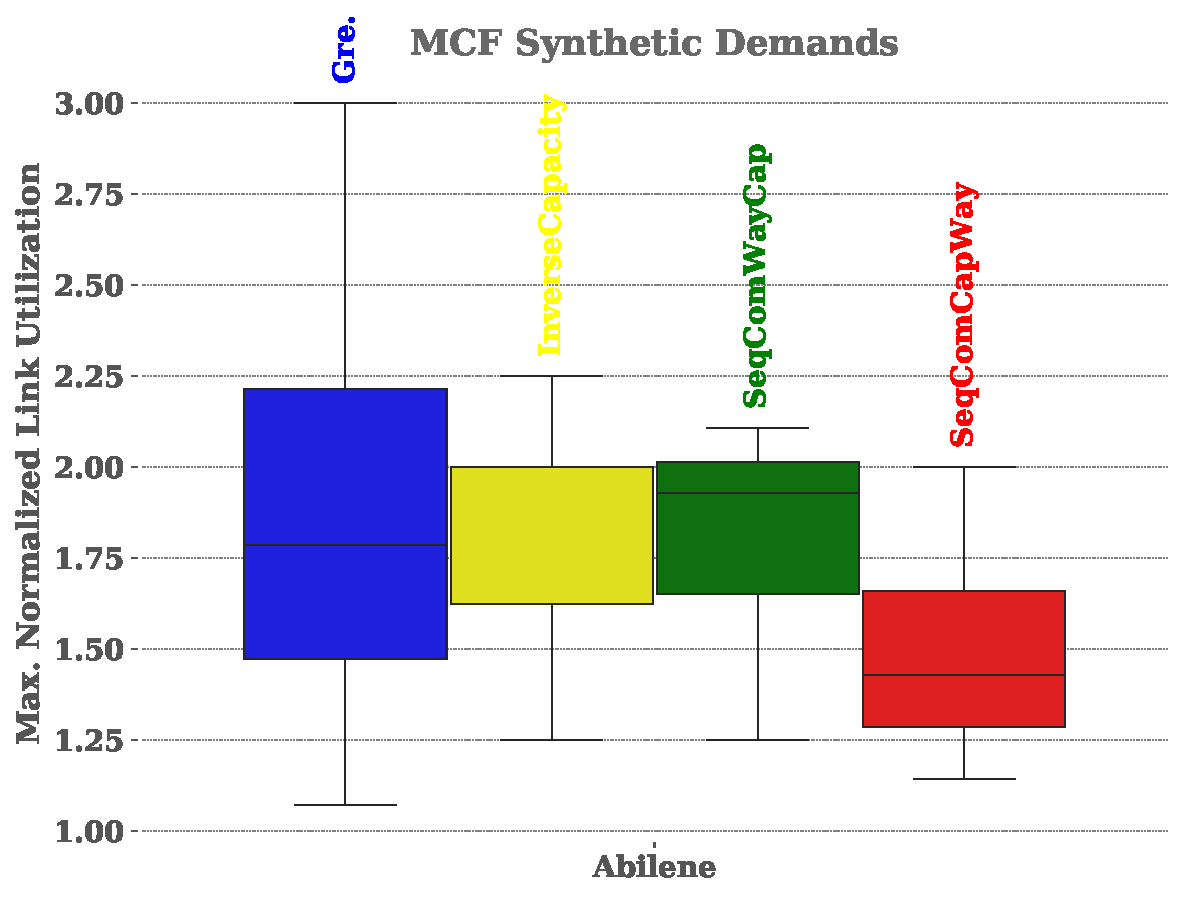
\includegraphics[width=\linewidth]{figures/pouria_all_algorithms_abilene.pdf}
\caption{Vergleich von vier Algorithmen mit synthetischen Anforderungen auf der Abilene-Topologie. Legende: \emph{greedy waypoints} in blau, \emph{inverse capacity} in gelb, SeqComWayCap in gr\"un, SeqComCapWay in rot.}
\label{fig:pouriaBoxplotSynthetic}
\end{figure}
% Das [h] kann weg, dann findet Tabelle automatisch den besten Platz
\begin{figure}
\centering
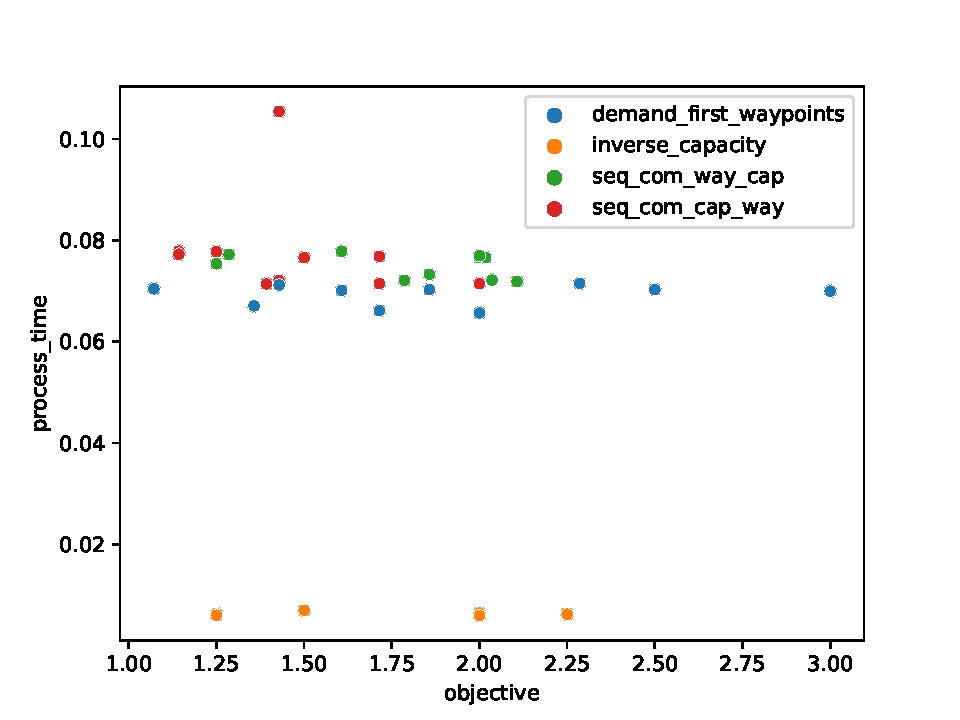
\includegraphics[width=\linewidth]{figures/pouria_colored_scatter_plot_results_all_algorithms.pdf}
\caption{Vergleich von vier Algorithmen mit syntetischen Anforderungen auf der Abilene-Topologie. Legende: \emph{greedy waypoints} in blau, \emph{inverse capacity} in gelb, SeqComWayCap in gr\"un, SeqComCapWay in rot.}
\label{fig:pouriaScatterSynthetic}
\end{figure}
% Das [h] kann weg, dann findet Tabelle automatisch den besten Platz
\begin{figure}
\centering
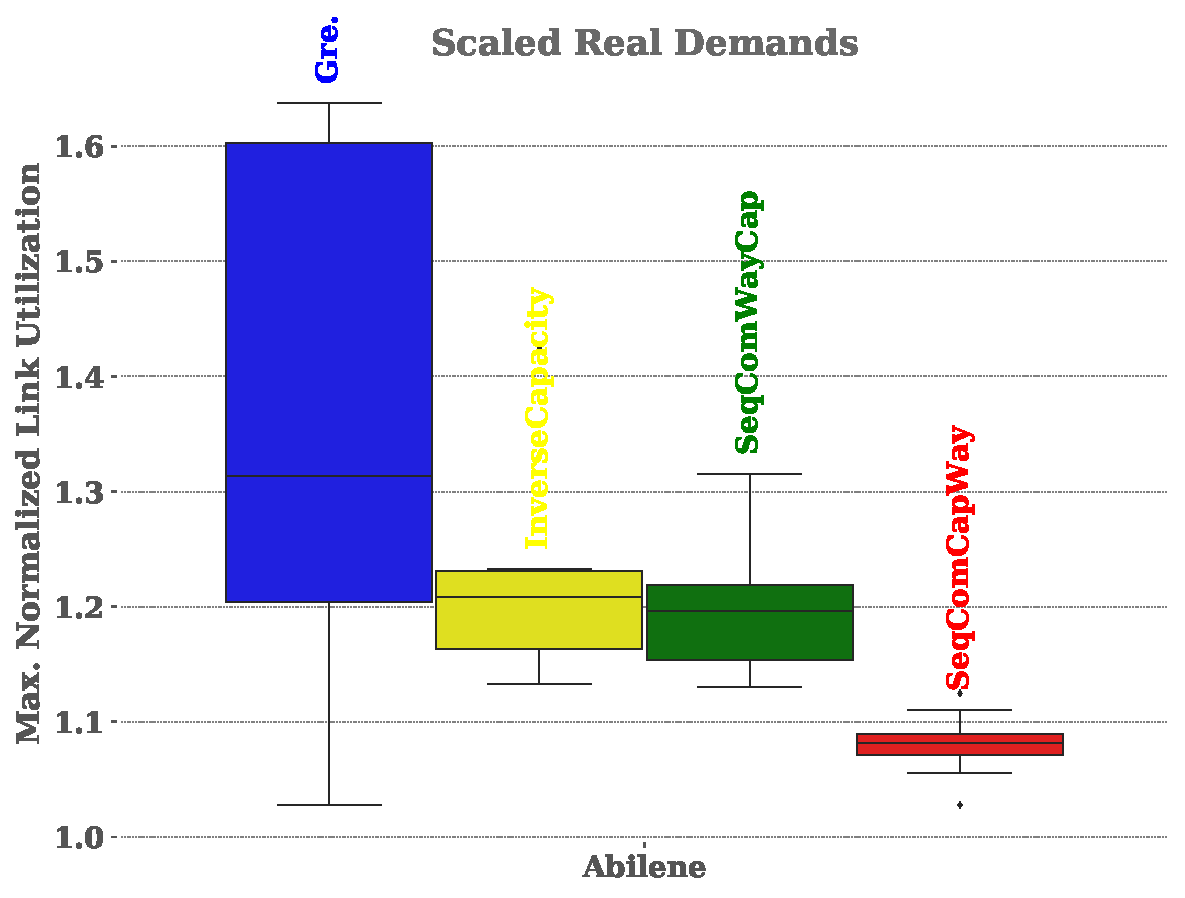
\includegraphics[width=\linewidth]{figures/pouria_real_demands.pdf}
\caption{Vergleich von vier Algorithmen mit realen Anforderungen auf der Abilene-Topologie. Legende: \emph{greedy waypoints} in blau, \emph{inverse capacity} in gelb, SeqComWayCap in gr\"un, SeqComCapWay in rot.}
\label{fig:pouriaBoxplotReal}
\end{figure}
% Das [h] kann weg, dann findet Tabelle automatisch den besten Platz
\begin{figure}
\centering
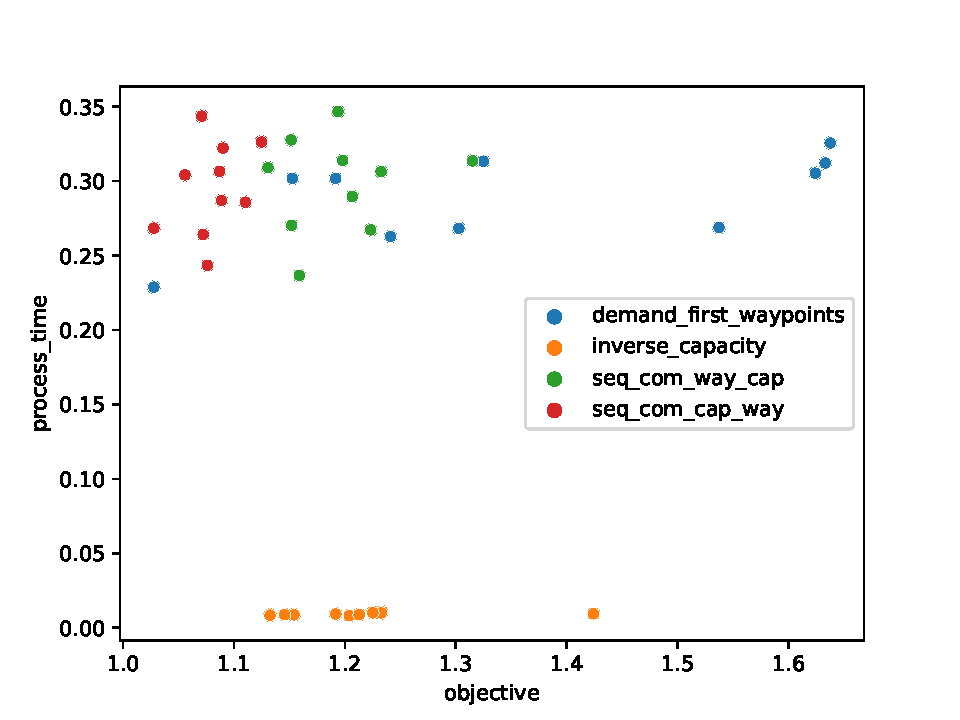
\includegraphics[width=\linewidth]{figures/pouria_colored_scatter_plot_results_real_demands.pdf}
\caption{Vergleich von vier Algorithmen mit syntetischen Anforderungen auf der Abilene-Topologie. Legende: \emph{greedy waypoints} in blau, \emph{inverse capacity} in gelb, SeqComWayCap in gr\"un, SeqComCapWay in rot.}
\label{fig:pouriaScatterReal}
\end{figure}
Die Abbildungen \ref{fig:pouriaBoxplotSynthetic} und \ref{fig:pouriaBoxplotReal} geben eine Antwort auf Frage 1.\newline
Sie zeigen, 
dass die sequentielle Kombination beider Algorithmen in beiden F\"allen mindestens genauso gut ist wie eines seiner Bestandteile. 
Im Fall von $SeqComCapWay$ ist dieser im Durchschnitt sogar besser als beide Algorithmen.
Dies l\"asst sich darauf zur\"uckf\"uhren, 
dass die Kantengewichte durch den \emph{inverse capacity}-\newline
Algorithmus zu Beginn verbessert werden 
und anschlie\ss end durch den zweiten Algorithmus weiter verbessert werden, falls m\"oglich.
Im Folgenden wird daher nur noch auf die sequentielle Kombination \emph{SeqComCapWay} (in rot) eingegangen.\newline
Die Abbildungen \ref{fig:pouriaScatterSynthetic} und \ref{fig:pouriaScatterReal} hingegen sind relevant f\"ur die Frage 2. 
Diese zeigen einen etwas genaueren Blick auf die Rechenergebnisse geplottet \"uber die daf\"ur ben\"otigte Zeit.
Hier kann auch direkt gesehen werden, dass \emph{inverse capacity} mit Abstand der schnellste hier verwendete Algorithmus ist.
Dies ist besonders vorteilhaft, da es bedeutet, 
dass die sequentielle Kombination aus \emph{inverse capacity} und \emph{greedy waypoints} kaum mehr Berechnungszeit ben\"otigt als \emph{greedy waypoints} alleine.
Somit konnte empirisch gezeigt werden, 
dass in diesem "vereinfachten" Beispiel die Kombination der oben genannten Algorithmen nicht nur im Durchschnitt bessere MLU-Ergebnisse liefert, 
sondern das auch in derselben Zeit erledigt.
Und somit l\"asst sich die Frage der Rechtfertigung auslagern.
In allen F\"allen, in denen der \emph{greedy waypoints}-Algorithmus gerechtfertigt ist,
ist auch die oben genannte Kombination gerechtfertigt.\newline
Da es aus Zeitgr\"unden sowie mangelnder Rechenressourcen nicht so einfach m\"oglich war,
diese Algorithmen auf sehr gro\ss en Tologien zu testen,
kann nicht mit Sicherheit gesagt, wie hoch die Berechnungszeit in Topologien mit 50 oder mehr Knoten wirklich ist.
Daher ist es schwer, diese Algorithmen (mit Ausnahme von \emph{inverse capacity} in solchen Topologien dynamisch zu verwenden.
% %%%%%%%%%%%%%%%%%%%%%%%%%%%%%%%%%%%%%%%%%%%%%%%%%%%%%%%%%%%%%%%%%%
% Kai
% %%%%%%%%%%%%%%%%%%%%%%%%%%%%%%%%%%%%%%%%%%%%%%%%%%%%%%%%%%%%%%%%%%
\subsubsection{Centrality-Metriken mit \emph{inverse capacity}}
Der Gedanken hier war, den Algorithmus \emph{inverse capacity}, der statisch auf der Topologie (also unabh\"angig von den demands) berechnet wird, mit Zentralit\"atswerten zu erweitern.

Ich habe mich f\"ur die Zentralit\"atswerte closeness-, eigenvector- und betweeness-Zentralit\"at entscheiden.
Im Folgenden werden nun die Zentralit\"atsmetriken definiert (Definitionen aus \cite{guide}), und dann erl\"autet warum diese ausgew\"ahlt wurden:

\begin{enumerate}
\item \textbf{Adjazenzmatrix}
Adjazenzmatrix \texttt{A} wird benutzt um einen Graphen als Matrix darzustellen.
Hierf\"ur gilt:
\[
a_{ik} = \begin{cases} 1 & \text{wenn Knoten i und k eine Kante verbindet}, \\ 0 & \text{sonst} \end{cases}
\]
\item \textbf{closeness-centrality}
Wie der Name bereits vermuten l\"asst, berechnet diese Metrik, 
wie nah ein Knoten allen anderen ist.
Die closeness-centrality $c_i$ des Knoten $i$:
\[
    c_i = \frac{1}{\sum_{j\neq i} H(\mathcal{P}_{i\rightarrow j})}
\]
$\mathcal{P}_{i\rightarrow j}$ ist der k\"urzeste Pfad von Knoten i nach Knoten j.
    
$H(\mathcal{P}_{i\rightarrow j})$ ist die Anzahl an Kanten, die genutzt werden m\"ussen, um von Knoten $i$ nach Knoten $j$ zu kommen.
    
Je h\"oher die closeness-Metrik, desto zentraler ist der Knoten im Graph. 
    
\item \textbf{betweenness-centrality}
Die betweenness-centrality gibt das Verh\"altnis aller k\"urzesten Wege, 
die durch einen Knoten $i$ f\"uhren, zur Menge aller k\"urzesten Wege an.
    
Die betweenness-centrality eines Knoten $i$:
\[
b_i = \sum_{s,t\in \mathcal{N}} \frac{|\mathcal{P}_{s\rightarrow t}(i)|}{|\mathcal{P}_{s\rightarrow t}|}
\]
wobei $|\mathcal{P}_{s\rightarrow t}|$ die Anzahl aller k\"urzesten Wege von $s$ nach $t$ ist und $|\mathcal{P}_{s\rightarrow t}(i)|$ die Anzahl dieser Wege, die durch den Knoten $i$ verlaufen. 
      
\item \textbf{eigenvector-centrality):}
     
 Die eigenvektor-centrality $x_i$ eines Knotens $i$ ist das $i$-te Element des Eigenvektors, 
 die dem gr\"o\ss ten Eigenwert $\lambda_1$ der Adjazenz-Matrix A entspricht.
     
Die Formel zur Berechnung lautet:
\[
x_i = \frac{1}{\lambda_1}\sum^N_{k=1}a_{ik}x_k
\]
     
Hat ein Knoten einen hohen eigenvektor-centrality, 
l\"asst sich folgern, dass der Knoten mit anderen wichtigen Knoten verbunden ist.

\end{enumerate}

Die closeness-centrality wurde gew\"ahlt, da die closeness aussagt wie vielen Kanten ein Knoten von allen anderen entfernt ist, daher potenziell viele Datenst\"orme durch diesen Knoten flie\ss en k\"onnen.
Die betweeness-centrality wurde gew\"ahlt, da Knoten mit hoher betweeness, an vielen k\"urzesten Wegen beteiligt sind, hier also das Risiko f\"ur Link \"uberlastung hoch ist.
Die eigenvector-centrality wurde gew\"ahlt, da eine hohe eigenvector-centrality darauf schlie\ss en l\"asst, dass der Knoten ein guter "Verteiler"-Knoten im Netz ist.

In der tats\"achlichen Implementierung wurden die centrality Berechnungen von NetworkKit benutzt, und dort zus\"atzlich noch normalisiert.

Um \emph{inverse capacity} mit den centrality Werten zu verrechnen wird folgende Formel genutzt (f\"ur die Kante von i nach j:
\begin{align*}
&new\_weight_{ij} =\\
&inverse capacity\_weight * \frac{CentralityNode_i + CentralityNode_j}{2}
\end{align*}
In \ref{fig:kai_p1_results} gibt es neben dem centralityInverseCapacity auch noch den centralityCapacity, dass ist der Algorithmus ohne \emph{inverse capacity}, also:
\[
new\_weight_{ij} = weight * \frac{CentralityNode_i + CentralityNode_j}{2}
\]
Diese d\"urften schlecht abschneiden, sind hier jedoch mit dabei, um den Unterschied zu unterstreichen.


%%Auswertung Projekt 1
\begin{figure}
\centering
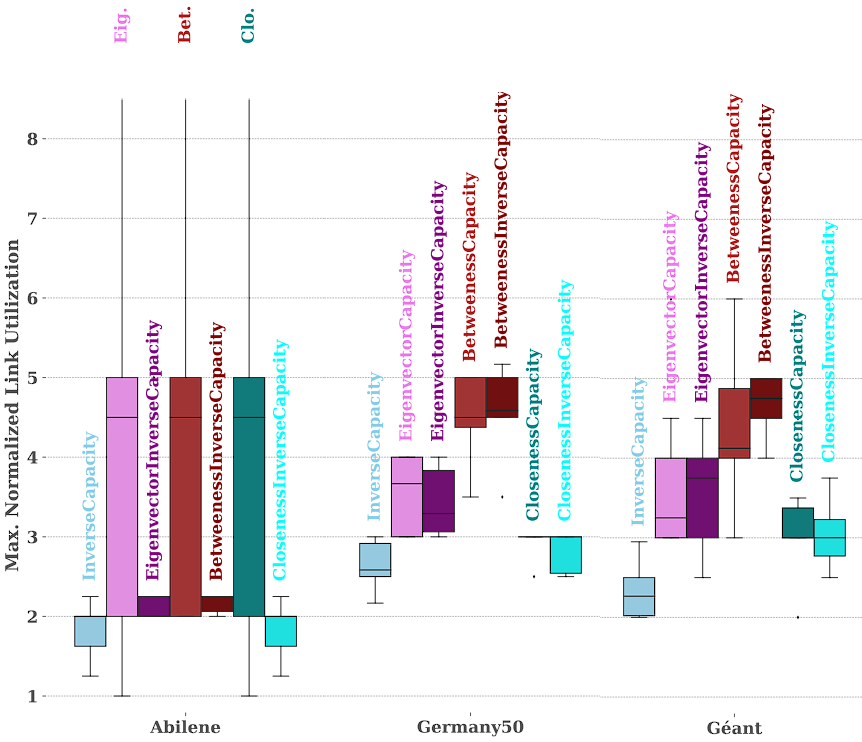
\includegraphics[width=\linewidth]{figures/kai_p1_results.png}
\caption{Ergebnisse f\"ur centrality-inverse-capacity}
\label{fig:kai_p1_results}
\end{figure}


Wie man in Abbildung \ref{fig:kai_p1_results} zu sehen ist, ist der neue Algorithmus keine Verbesserung auf den getesteten Topologien.
Am schlechtesten schneidet hier der Algorithmus mit der betweeness centrality ab, dicht gefolgt von der eigenvector centrality.
Die closeness centrality schneidet mit am besten ab und ist im Beispiel f\"ur "Abilene" gleich auf mit \emph{inverse capacity}.
Die Algorithmen ohne \emph{inverse capacity} sind, schlechter, jedoch (abgesehen von Abilene) nah an den anderen Algorithmen dran.

Die schlechtere Performance kann dadurch erkl\"art werden, dass die weights der Kanten bei reinem \emph{inverse capacity}, zwei k\"urzeste Wege zwischen zwei Knoten entstehen lassen, und diese durch die centralities dann, durch die neue Gewichtung, nur noch einen k\"urzesten Weg haben.
Dadurch werden dann einzelne Links \"uberlastet und die MLU wird schlechter.
% %%%%%%%%%%%%%%%%%%%%%%%%%%%%%%%%%%%%%%%%%%%%%%%%%%%%%%%%%%%%%%%%%%
% Naveed
% %%%%%%%%%%%%%%%%%%%%%%%%%%%%%%%%%%%%%%%%%%%%%%%%%%%%%%%%%%%%%%%%%%
\subsubsection{Sequential Combination aus OSPF und Uniform Weights}
\begin{figure}
\centering
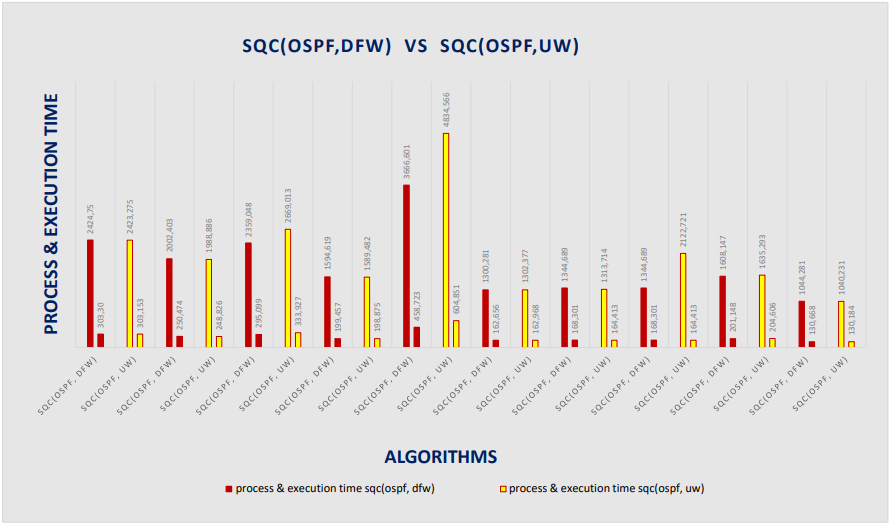
\includegraphics[width=\linewidth]{figures/naveed_p1.png}
\caption{Plotergebnisse}
\label{fig:naveed_p1}
\end{figure}
Der zentrale Gedanke dieses  Algorithmus bestand darin, 
im Rahmen des ersten Projekts die urspr\"ungliche Kombination aus OSPF und Demand First Waypoint(DFW)  zu optimieren, 
indem der DFW durch den Uniform Weights ersetzt wurde. 
Beide Algorithmen haben das Ziel, die Netzwerk\"uberlastung zu minimieren, indem sie die Linkgewichte anpassen. 
Jedoch unterscheiden sie sich in ihrer Herangehensweise an das Traffic Engineering.\newline
Der DFW-Algorithmus fokussiert sich darauf, den Verkehr zu spezifischen Zwischenpunkten im Netzwerk, 
sogenannten Waypoints, zu leiten, um die Verkehrslast auszugleichen und Stau zu vermeiden. 
Auf der anderen Seite zielt der UW-Algorithmus darauf ab, den Verkehr gleichm\"a\ss ig \"uber das gesamte Netzwerk zu verteilen.\newline
Das Ziel bestand darin herauszufinden, 
welche Kombination dieser Algorithmen in Bezug auf die \emph{Maximum Link Utilization} (MLU) die besseren Ergebnisse f\"ur den Datenverkehr im Netwerk liefert.\newline
Die Tests\footnote{\url{https://github.com/fruitiestPunch/FaPro\_P1}} f\"ur beide Algorithmen wurden erfolgreich durchgef\"uhrt, Allerdings gab es Schwierigkeiten beim Plotten der Ergebnisse aufgrund zahlreicher Fehlermeldungen, 
und aufgrund mangelder Erfahrung mit Python fiel es schwer, diese Fehler zu beheben.\newline
Dennoch wurden einige Ergebnisse wie die Prozesszeit und Ausf\"uhrungszeit beider Algorithmen manuell zusammengefasst, 
wie in Abbildung \ref{fig:naveed_p1} dargetellt. 
Die Auswertung zeigt, dass in einigen F\"allen die Kombination aus OSPF und DFW besser abschneidet, 
w\"ahrend in anderen F\"allen die Kombination aus OSPF und UW bessere Ergebnisse liefert. 
Im Durchschnitt kann man sagen, dass die Kombination von OSPF und DFW \"ahnlich gute Leistung erbringt wie OSPF mit UW.\newline
OSPF mit UW bietet folgende Merkmale:
\begin{enumerate}
\item Einfache Konfiguration und Verwaltung des Routers, da alle Verbindungen die gleiche Kostenmetrik haben.
\item Gleichm\"a\ss ige Lastverteilung \"uber das Netzwerk, da alle Verbindungen als gleichwertig behandelt warden.
\item Begrenzte Optimierungsf\"ahigkeit: 
durch die Verwendung einheitlicher Gewichte kann OSPF mit UW  keine spezifischen Leistungsmerkmale oder Netzwerkanforderungen ber\"ucksichtigen. 
Dies kann in einigen Anwendungsf\"allen zu Suboptimalit\"at in Bezug auf Bandbreite,
Verz\"ogerung oder andere wichtige Faktoren f\"uhren.
\item Es ist nicht empfohlen in komplexen Netzwerken mit unterschiedlichen Leistungseigenschaften der Verbindungen, 
da die einheitliche Gewichte nicht auf die individuellen Anforderungen reagieren k\"onnen.
\item Empfohlen in Netzwerken mit homogenen Verbindungen, bei denen keine signifikanten Unterschiede in den Leistungseigenschaften bestehen.
\end{enumerate}
Also wenn eine dynamische Anpassung des Routings, Ressourceneffizienz und die F\"ahigkeit, 
auf Ver\"anderungen zu reagieren, wichtig sind, kann OSPF mit DFW geeigent sein. 
Wenn hingegen eine einfache Konfiguration und gleichm\"a\ss ige Lastverteilung gew\"unscht sind, kann OSPF mit UW angemessen sein.
% %%%%%%%%%%%%%%%%%%%%%%%%%%%%%%%%%%%%%%%%%%%%%%%%%%%%%%%%%%%%%%%%%%
% Projekt 2
% %%%%%%%%%%%%%%%%%%%%%%%%%%%%%%%%%%%%%%%%%%%%%%%%%%%%%%%%%%%%%%%%%%
\subsection{Experimente zu Projekt 2}
In diesem Projekt ging es darum, die eigene algorithmische Idee zu nehmen und in einem virtuellen Netzwerk\footnote{\url{https://github.com/nikolaussuess/nanonet}, siehe Abschnitt \ref{sec:resouces}} zu testen. 
Dieses Projekt wurde ebenfalls mithilfe eines bereits existierenden Repositories\footnote{\url{https://github.com/fruitiestPunch/FaPro_P2}, siehe Abschnitt \ref{sec:resouces}} bearbeitet.
% %%%%%%%%%%%%%%%%%%%%%%%%%%%%%%%%%%%%%%%%%%%%%%%%%%%%%%%%%%%%%%%%%%
% Pouria
% %%%%%%%%%%%%%%%%%%%%%%%%%%%%%%%%%%%%%%%%%%%%%%%%%%%%%%%%%%%%%%%%%%
\subsubsection{Sequential combination aus \emph{inverse capacity} und \emph{demand first waypoints}}
\label{sec:seq_com_p2}
Zum Testen dieses Algorithmus wurde eine vereinfachte Topologie mit wenigen Anforderungen erstellt.
In Abbildung \ref{fig:pouriaSimpleTopology} ist die finale Topologie zu sehen, 
wobei hier bereits der \emph{inverse capacity}-Algorithmus darauf ausgef\"uhrt wurde.
In der Tabelle \ref{tab:pouriaSimpleTopology} sind die beiden Anforderungen sowie deren Start- und Endknoten angegeben.
In diesem Projekt kam es zu einigen Problemen, die durch die Rechenst\"arke der genutzten Hardware verschuldet wurden.
Abschnitt \ref{sec:alt_boxplot} befasst sich st\"arker mit diesem Punkt und dessen Auswirkungen.
Abbildung \ref{fig:pouria_boxplot_no_boxes} zeigt dabei die MLU-Werte von zwei Algorithmen im Vergleich.
Hierf\"ur wurden der Weights-Algorithmus und der sequentielle Kombinations aus \emph{inverse capacity} und \emph{demand first waypoints} miteinander verglichen.\newline
Anhand der Form der Boxplots ist zu erkennen, dass es keine bis minimale Streuung in den finalen Ergebnissen gab.
Im Allgemeinen schneiden beide Algorithmen gleich gut ab, denn bei in beiden F\"allen liegt die durchschnittliche MLU bei unter 2.
Allerdings ist in Abbildung \ref{fig:pouria_boxplot_no_boxes} auch zu erkennen, dass beide Ausrei\ss er enthalten,
wobei der Ausrei\ss er vom Weights-Algorithmus wesentlich besser liegt, als der andere.
Es wird vermutet, dass die starke Spezialisierung des SC-Algorthmus auf der gegebenen Topologie dazu f\"uhrt, 
dass er im Allgemeinen sehr gute MLU-Ergebnisse liefert,
aber im \emph{worst-case} nicht so gut abschenidet.
Im Vergleich liefert Weights-Algorithmus generell konsistent \"ahnliche Ergebnisse,
sodass er im \emph{worst-case} dennoch nicht ganz schlecht ausgeht.
\begin{figure}
\centering
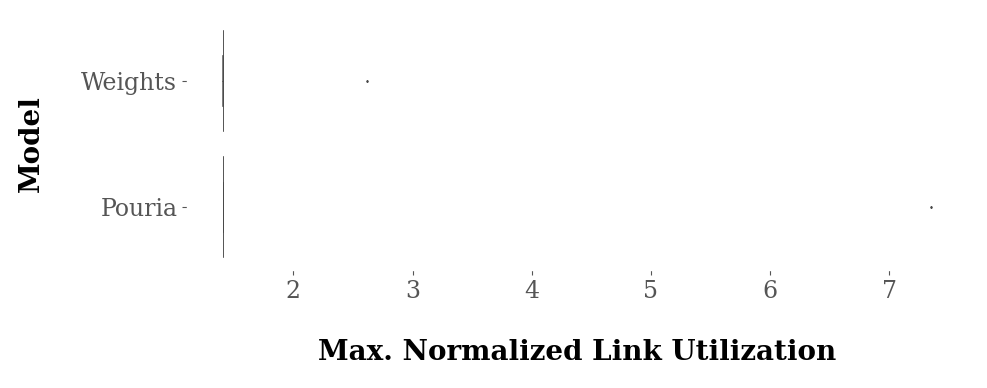
\includegraphics[width=\linewidth]{figures/pouria_boxplot_no_boxes.png}
\caption{Vergleich von zwei Algorithmen als Boxplotdiagramme.}
\label{fig:pouria_boxplot_no_boxes}
\end{figure}
% Das [h] kann weg, dann findet Tabelle automatisch den besten Platz
\begin{figure}
\centering
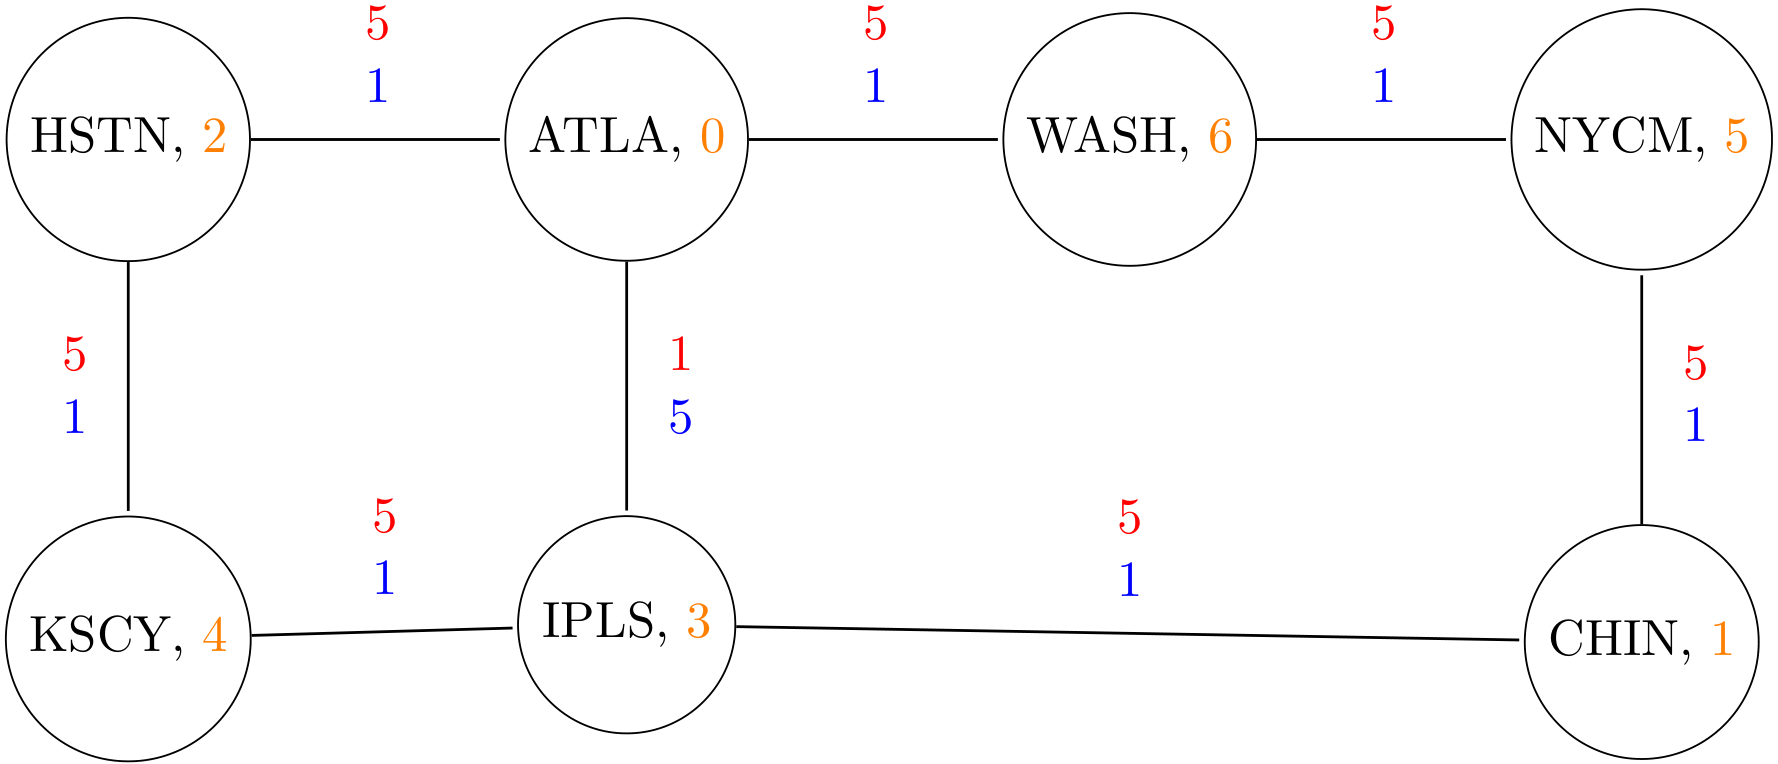
\includegraphics[width=\linewidth]{figures/pouria_simple_topology.png}
\caption{Vereinfachte Netzwerktopologie [Anlehnung an Abilene]. Legende: Kapazit\"aten in rot, Gewichte in blau.}
\label{fig:pouriaSimpleTopology}
\end{figure}
% Das [h] kann weg, dann findet Tabelle automatisch den besten Platz
\begin{table}
\caption{Vereinfachte Anforderungstabelle. Vollst\"andige Tabelle unter \url{https://github.com/fruitiestPunch/FaPro_P2/tree/master/pouria/network_origin.pdf}}
\label{tab:pouriaSimpleTopology}
\begin{tabular}{cccc}
\toprule
$\downarrow$ von, nach $\rightarrow$&IPLS&WASH&$\cdots$\\
\midrule
ATLA & 5 & &\\
IPLS & & 7 & \\
$\vdots$ & & & \\
\bottomrule
\end{tabular}
\end{table}
% %%%%%%%%%%%%%%%%%%%%%%%%%%%%%%%%%%%%%%%%%%%%%%%%%%%%%%%%%%%%%%%%%%
% Kai
% %%%%%%%%%%%%%%%%%%%%%%%%%%%%%%%%%%%%%%%%%%%%%%%%%%%%%%%%%%%%%%%%%%
\subsubsection{Centrality-Metriken mit \emph{inverse capacity}}
\begin{figure}
\centering
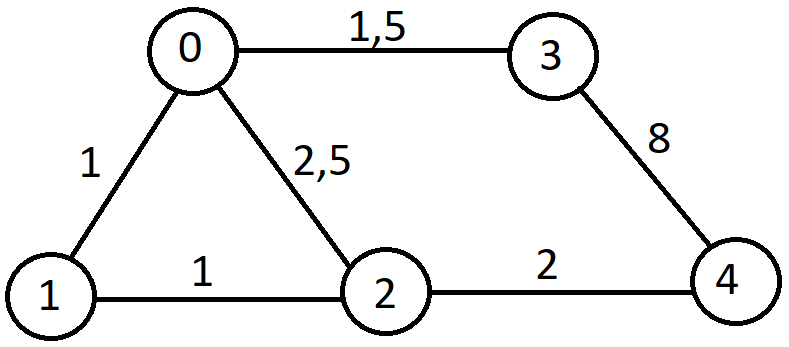
\includegraphics[width=\linewidth]{figures/kai_p2_baseTopo.png}
\caption{Topologie f\"ur die Tests des Algorithmus centrality Metriken mit \emph{inverse capacity}}
\label{fig:kai_p2_baseTopo}
\end{figure}
Die Topologie f\"ur die Tests der centrality Metriken mit \emph{inverse capacity} ist die in Abbildung \ref{fig:kai_p2_baseTopo}.
Es gibt zwei Demands, einmal von 0 nach 4 mit Gr\"o\ss e 1, und einmal von 3 nach 4 mit Gr\"o\ss e 8.
Au\ss erdem wurde hier nur die centrality Metrik closeness benutzt, da diese im ersten Projekt am besten der drei Metriken abgeschlossen hat.

Warum diese Topologie genutzt wurde, wird klar wenn man sich die Ergebnisse anschaut.
Wie man in Abbildung \ref{fig:kai_p2_results} sehen kann, performt auf dieser Topologie der Algorithmus besser als \emph{inverse capacity}.
Der Grund daf\"ur wird in Abbildung \ref{fig:kai_p2_AdTopo} verdeutlicht.
\emph{inverse capacity} schickt beide Demands \"uber die Kante zwischen 3 und 4, dadurch wird diese \"uberlastet.
\emph{inverse capacity} mit der closeness Metrik schick ein Demand von 3 nach 4 und den anderen \"uber 0 nach 2 nach 4 und verhindert dadurch die \"uberlastung.
\begin{figure}
\centering
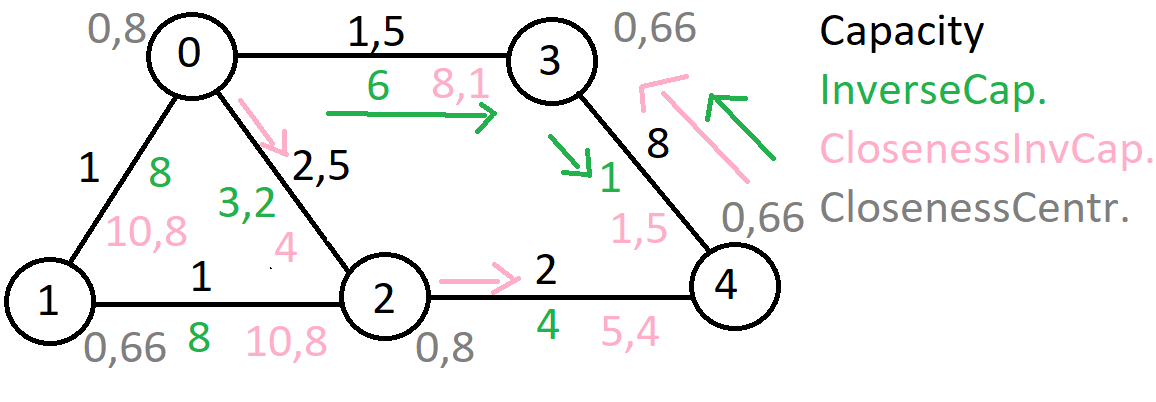
\includegraphics[width=\linewidth]{figures/kai_p2_TopoAd.png}
\caption{Topologie mit ausgerechneten Werte, Pfeile geben die jeweils genommenen Pfade an}
\label{fig:kai_p2_AdTopo}
\end{figure}
\begin{figure}
\centering
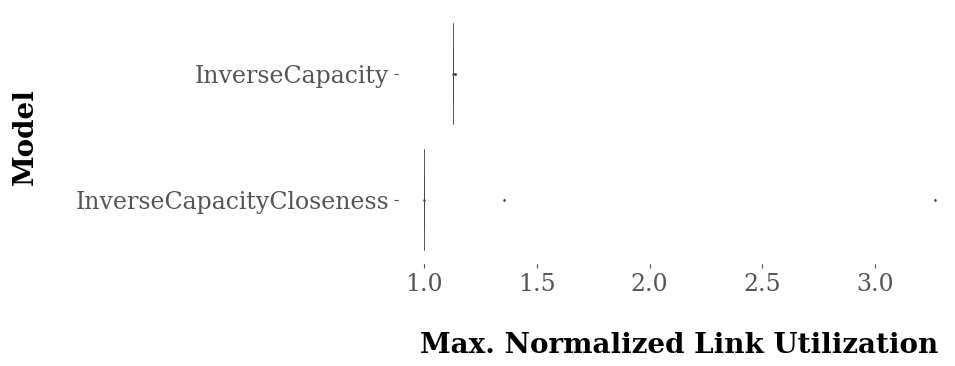
\includegraphics[width=\linewidth]{figures/kai_p2_results.png}
\caption{Ergebnisse f\"ur Algorithmus centrality Metriken mit \emph{inverse capacity}}
\label{fig:kai_p2_results}
\end{figure}
% %%%%%%%%%%%%%%%%%%%%%%%%%%%%%%%%%%%%%%%%%%%%%%%%%%%%%%%%%%%%%%%%%%
% Naveed
% %%%%%%%%%%%%%%%%%%%%%%%%%%%%%%%%%%%%%%%%%%%%%%%%%%%%%%%%%%%%%%%%%%
\subsubsection{Sequential Combination aus OSPF und Uniform Weights}
Um den Algorithmus in Nanonet zu testen, wurde eine Topologie1 erstellt, 
die 5 Knoten umfasst, wie in Abbildung \ref{fig:naveed_p2_graph} dargestellt. 
Dabei wurden allen Kanten gleichm\"a\ss ige Gewichtungen zugewiesen. 
Anschlie\ss end wurden Demands von Knoten 0 zu Knoten 4 gesendet. 
Um sicherzustellen, dass alle verf\"ugbaren Wege von 0 zu Knoten 4  genutzt werden,
wurden Knoten 1 und 3 als sogenannte Waypoints hinzugef\"ugt.
In Abbildung \ref{fig:naveed_p2_boxplot} ist der Vergleich zwischen JoinUW (oben) und der Sequential Combination aus OSPF und UW (unten) zu sehen.
\begin{figure}
\centering
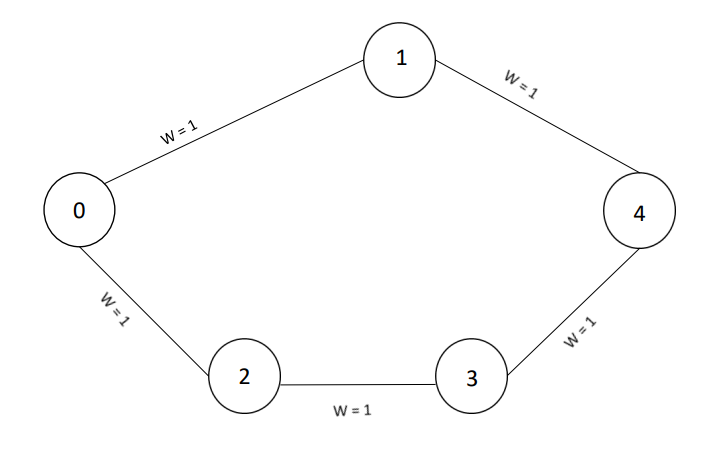
\includegraphics[width=\linewidth]{figures/naveed_p2_graph.png}
\caption{Plotergebnisse}
\label{fig:naveed_p2_graph}
\end{figure}
\begin{figure}
\centering
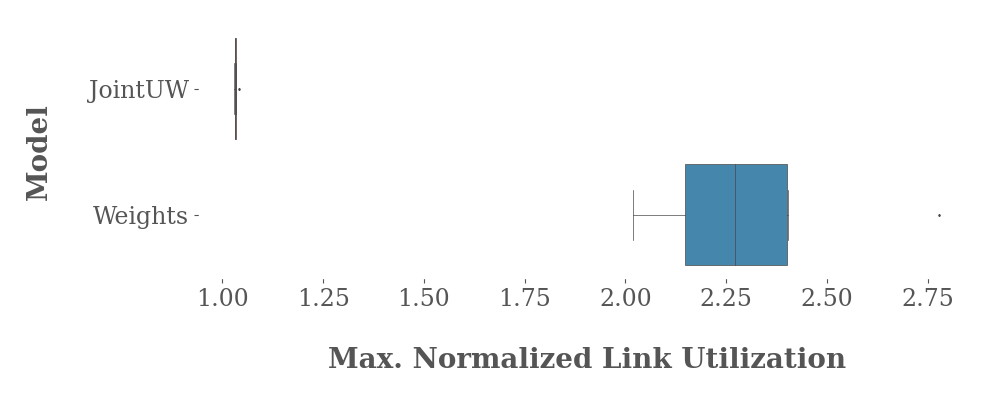
\includegraphics[width=\linewidth]{figures/naveed_p2_boxplot.png}
\caption{Topologie}
\label{fig:naveed_p2_boxplot}
\end{figure}

% %%%%%%%%%%%%%%%%%%%%%%%%%%%%%%%%%%%%%%%%%%%%%%%%%%%%%%%%%%%%%%%%%%
% Replikation
% %%%%%%%%%%%%%%%%%%%%%%%%%%%%%%%%%%%%%%%%%%%%%%%%%%%%%%%%%%%%%%%%%%
\section{Replikation}
Im Folgenden werden die Ergebnisse und Einsichten der Replikationen von Gruppe 2 vorgestellt.
% %%%%%%%%%%%%%%%%%%%%%%%%%%%%%%%%%%%%%%%%%%%%%%%%%%%%%%%%%%%%%%%%%%
% Projekt 1
% %%%%%%%%%%%%%%%%%%%%%%%%%%%%%%%%%%%%%%%%%%%%%%%%%%%%%%%%%%%%%%%%%%
\subsection{Replikation zu Projekt 1}
Die Replikation von diesem Projekt\footnote{\url{https://github.com/kohlbold/FpRouting}} war zu Beginn leider etwas schwierig, weil in beiden F\"allen Abh\"angigkeiten fehlten.
Ein gro\ss es Problem beim Replizieren des Deep-Learning-Projekts war, dass sich der Prozess nach einer Weile selbstst\"andig beendet hat.
Die Vermutung liegt nahe, dass der Rechenaufwand so hoch war, dass der Rechner ab einem bestimmten Zeitpunkt den Prozess selbst beendet hat.
Ein weiteres Problem beim Replizieren waren die Fehlermeldungen und Abbr\"uche beim Plotten. 
\begin{figure}
\centering
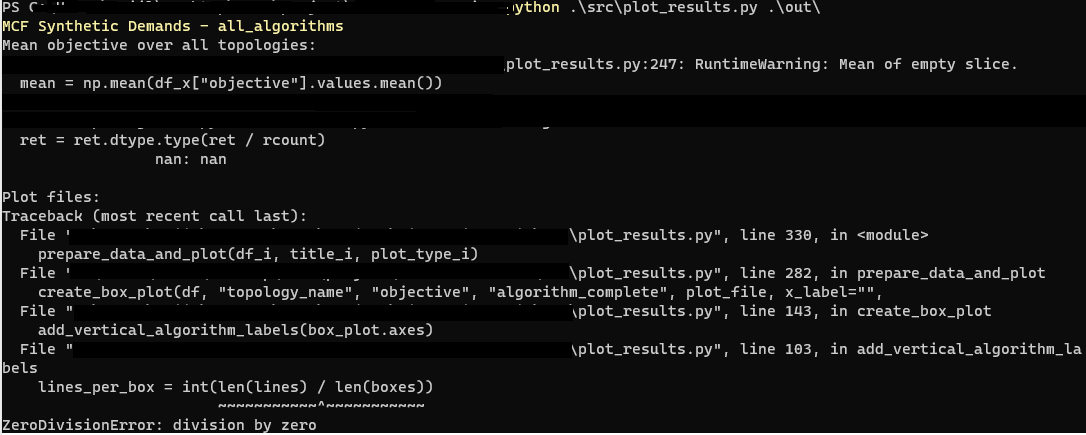
\includegraphics[width=\linewidth]{figures/repl_p1_plottererror.png}
\caption{Plotting-Fehlermeldung im Terminal}
\label{fig:repl_p1_plottererrror}
\end{figure}
Diesem und \"ahnlichen Fehlern sind wir bei unser Bearbeitung ebenfalls begegnet und die Behebung hat sich als au\ss erordentlich schwierig erwiesen, weil dieser "Plottererror" innerhalb einer Python-Bibliothek liegt.
Abbildung \ref{fig:repl_p1_plottererrror} zeigt einen solchen Fehler,
welcher sich hartn\"ackig auch nach einigen Anpassungsversuchen weiterhin erhalten hat.
% %%%%%%%%%%%%%%%%%%%%%%%%%%%%%%%%%%%%%%%%%%%%%%%%%%%%%%%%%%%%%%%%%%
% Replikation
% %%%%%%%%%%%%%%%%%%%%%%%%%%%%%%%%%%%%%%%%%%%%%%%%%%%%%%%%%%%%%%%%%%
\subsection{Replikation zu Projekt 2}
Die Replikation des Codes\footnote{\url{https://github.com/kohlbold/FPRouting2}} aus Gruppe 2 lief im Allgemeinen problemlos, wie die Abbildungen \ref{fig:repl_p2_daniel2} und \ref{fig:repl_p2_zixiang_10} zeigen.
\begin{figure}
\centering
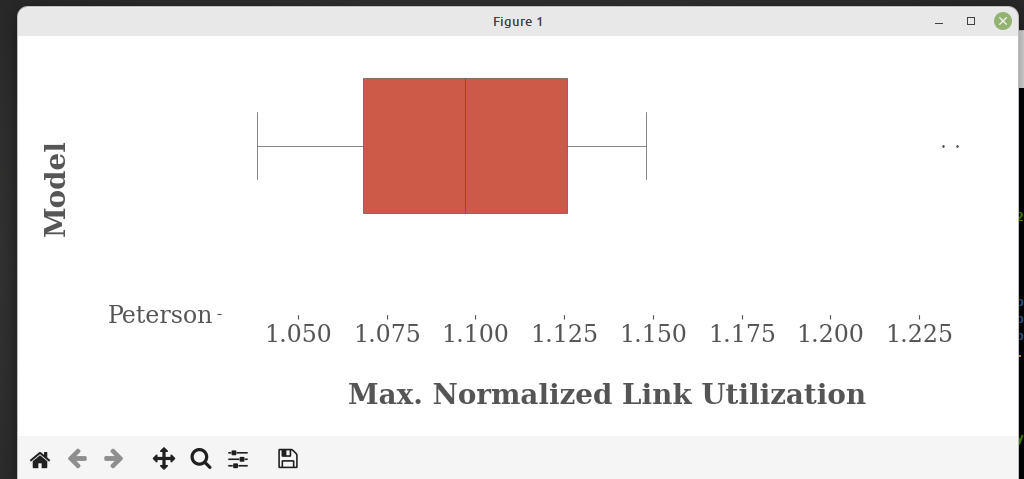
\includegraphics[width=\linewidth]{figures/repl_p2_daniel2.png}
\caption{Ergebnisdiagramm des Codes von Gruppe 2}
\label{fig:repl_p2_daniel2}
\end{figure}
\begin{figure}
\centering
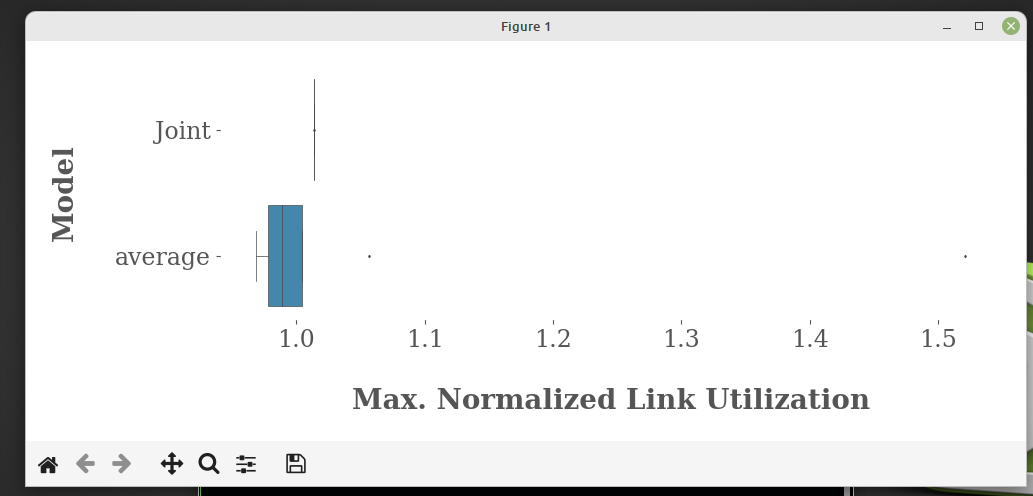
\includegraphics[width=\linewidth]{figures/repl_p2_zixiang_10.png}
\caption{Ergebnisdiagramm des Codes von Gruppe 2}
\label{fig:repl_p2_zixiang_10}
\end{figure}
Ein Problem, welches auch innerhalb unserer Gruppe aufgetaucht ist,
waren die identischen Werte nach Beendigung der \emph{nanonet\_batch.py}-Datei.
Wie bereits in Abschnitt \ref{sec:seq_com_p2} erw\"ahnt, liegt dieses Problem vermutlich an mangelnder Rechenleistung w\"ahrend des Berechnungsprozesses.
Nach wiederholtem Ausf\"uhren des Codes konnte dieses Problem jedoch behoben werden.
\begin{figure}
\centering
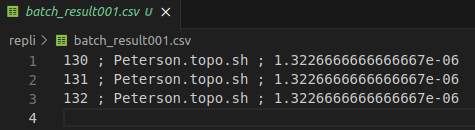
\includegraphics[width=\linewidth]{figures/repl_p2_daniel1.png}
\caption{Ergebnis-CSV-Datei mit identischen MLU-Werten in jeder Zeile}
\label{fig:repl_p2_daniel1}
\end{figure}

% %%%%%%%%%%%%%%%%%%%%%%%%%%%%%%%%%%%%%%%%%%%%%%%%%%%%%%%%%%%%%%%%%%
% Zusammenfassung
% %%%%%%%%%%%%%%%%%%%%%%%%%%%%%%%%%%%%%%%%%%%%%%%%%%%%%%%%%%%%%%%%%%
\section{Zusammenfassung}
Es kann gesagt werden, dass wir w\"ahrend des Fachprojekts vieles lernen konnten, 
insbesondere Dinge, die nicht notwendigerweise im Stundenplan stehen, 
aber gerade auf der akademischen Laufbahn als Standard angesehen werden.
Das Nachstellen einer wissenschaftlichen Arbeit hat sich als nicht-trivial erwiesen 
und das obwohl diese Arbeit f\"ur ihre hohe Reproduzierbarkeit ausgezeichnet wurde.
Dies l\"asst leider nur auf eine Folgerung schlie\ss en; viele andere wissenschaftlichen Arbeiten lassen sich viel schwerer oder gar nicht nachstellen. 
W\"ahrend des Replizierens der Projekte der anderen Gruppen war es ebenfall \"uberraschend, 
das selbst wenn unsere Gruppen alle an denselbem Hauptprojekt gearbeitet haben 
und theoretisch alle dieselben Pakete verwendeten, 
es manchmal dennoch zu Replikationsschwierigkeiten kam.
Allerdings war es auch eine sch\"one Erfahrung in einer Gruppe an so einem Projekt zu sitzen 
und die Probleme intern sowie mit den anderen Gruppen besprechen zu k\"onnen.
Das hat nicht nur zu einem gr\"o\ss eren Zusammengeh\"origkeitsgef\"uhl gef\"uhrt,
sondern wir haben auch gelernt, kollaborativ gemeinsame Schwierigkeiten zu l\"osen. 

% %%%%%%%%%%%%%%%%%%%%%%%%%%%%%%%%%%%%%%%%%%%%%%%%%%%%%%%%%%%%%%%%%%
% Ausblick
% %%%%%%%%%%%%%%%%%%%%%%%%%%%%%%%%%%%%%%%%%%%%%%%%%%%%%%%%%%%%%%%%%%
\section{Ausblick}
Aufgrund der relativ kurzen Bearbeitungszeit und den begrenzten Rechenkapazit\"aten unserer eigenen Computer war es etwas schwer, unsere Algorithmen, insbesondere in Projekt 2, auf gro\ss en Topologien zu testen.
Dies kann dazu f\"uhren, dass bestimmt Effekte wie Datenstaus, welche gerade in gro\ss en Topologien auftauchen, in kleinen kaum oder gar nicht vorkommen.

\begin{acks}
Vielen Dank an Marvin f\"ur seine Hilfe und Geduld mit unseren Problemen. Ohne seine Hilfe w\"are das alles in der kurzen Zeit sehr viel schwieriger gewesen.
\end{acks}

% %%%%%%%%%%%%%%%%%%%%%%%%%%%%%%%%%%%%%%%%%%%%%%%%%%%%%%%%%%%%%%%%%%
% Literatur
% %%%%%%%%%%%%%%%%%%%%%%%%%%%%%%%%%%%%%%%%%%%%%%%%%%%%%%%%%%%%%%%%%%
\bibliographystyle{ACM-Reference-Format}
\bibliography{fapro_bib}

% %%%%%%%%%%%%%%%%%%%%%%%%%%%%%%%%%%%%%%%%%%%%%%%%%%%%%%%%%%%%%%%%%%
% Appendix
% %%%%%%%%%%%%%%%%%%%%%%%%%%%%%%%%%%%%%%%%%%%%%%%%%%%%%%%%%%%%%%%%%%
\appendix
% %%%%%%%%%%%%%%%%%%%%%%%%%%%%%%%%%%%%%%%%%%%%%%%%%%%%%%%%%%%%%%%%%%
% Onlineressourcen
% %%%%%%%%%%%%%%%%%%%%%%%%%%%%%%%%%%%%%%%%%%%%%%%%%%%%%%%%%%%%%%%%%%
\section{Onlineressourcen}
\label{sec:resouces}
Im Rahmen dieses Fachprojekts wurden drei \"offentliche Repositories als Hauptquellen verwendet. Die ersten beiden Repositories\newline
\url{https://github.com/fruitiestPunch/FaPro_P1} und \newline
\url{https://github.com/fruitiestPunch/FaPro_P2}, welche \emph{forks} von\newline
\url{https://github.com/tfenz/TE_SR_WAN_simulation} und \newline
\url{https://github.com/nikolaussuess/TE_SR_experiments_2021}\newline
sind. Die dritte Hauptquelle stellt \url{https://github.com/nikolaussuess/nanonet} dar, welche zur Erstellung von vom Projekt les- und interpretierbaren Netzwerktopologiedaten verwendet wurde.

% %%%%%%%%%%%%%%%%%%%%%%%%%%%%%%%%%%%%%%%%%%%%%%%%%%%%%%%%%%%%%%%%%%
% Alternativer Boxplot
% %%%%%%%%%%%%%%%%%%%%%%%%%%%%%%%%%%%%%%%%%%%%%%%%%%%%%%%%%%%%%%%%%%
\section{Alternativer Boxplot}
\label{sec:alt_boxplot}
\begin{figure}
\centering
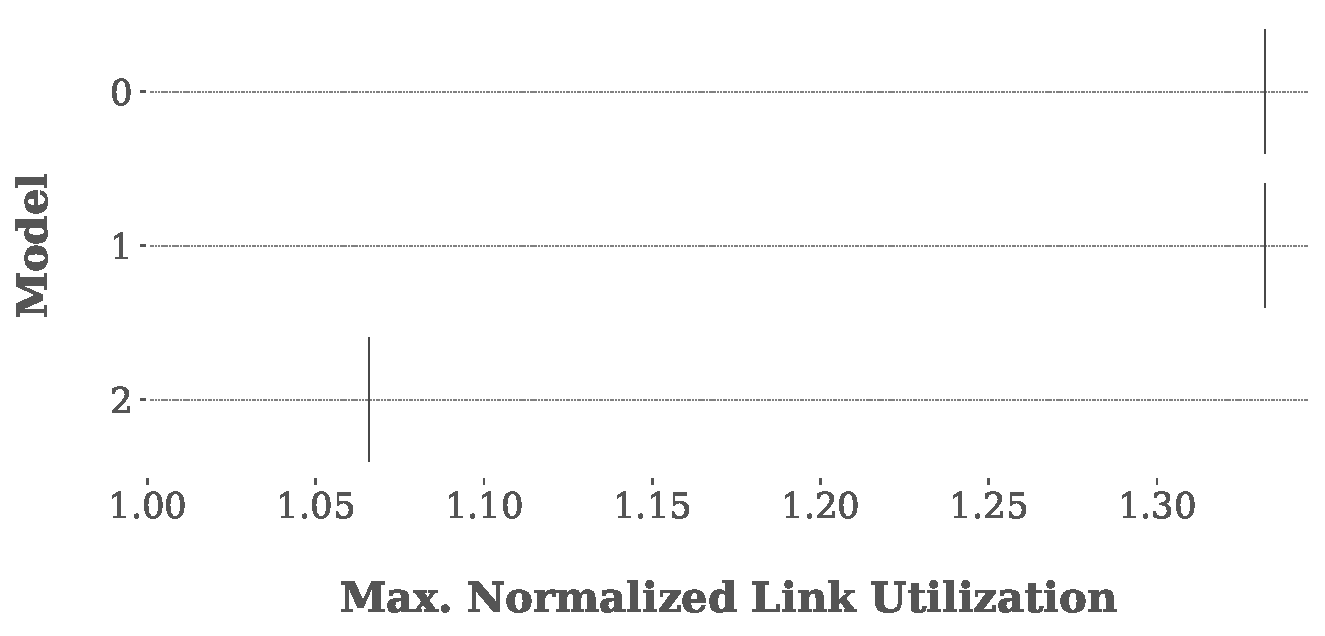
\includegraphics[width=\linewidth]{figures/pouria_boxplot_no_real_results.pdf}
\caption{Vergleich von drei Algorithmen als Boxplotdiagramme. Legende: 0 = Joint, 1 = Weights, 2 = Pouria.}
\label{fig:pouria_boxplot_no_real_results}
\end{figure}
Die Timeouts in den Experimenten von Projekt 2 haben zu einigen Problemen gef\"uhrt.
Speziell im Falle von Abschnitt \ref{sec:seq_com_p2} war der Rechner, 
auf dem der dortige Algorithmus getestet wurde,
wesentlich leistungsschw\"acher (4GB RAM) als die anderen Rechner.
Daher wird vermutet, 
dass die Timeouts
\footnote{\url{https://github.com/nikolaussuess/nanonet}, siehe Abschnitt \ref{sec:resouces}}
\footnote{\emph{nanonet\_batch.py} aus \url{https://github.com/fruitiestPunch/FaPro_P2}, siehe Abschnitt \ref{sec:resouces}}
\begin{verbatim}
  at now+2min
\end{verbatim}
und 
\begin{verbatim}
  sleep(8 * 60)
\end{verbatim}
nicht ausgereicht haben, sodass einige der Prozesse fr\"uhzeitig abgerbochen wurden.
Abbildung \ref{fig:pouria_boxplot_no_real_results} zeigt dabei die MLU-Werte aller drei Algorithmen im Vergleich.
Die Tatsache, dass die Boxplots hier nur als Striche dargestellt werden, weist daraufhin, dass es keine Streuung in den finalen Ergebnissen gab,
was auf das fr\"uhzeitige Abbrechen einiger Rechenprozesse zur\"uckgef\"uhrt werden kann.
% bug in the acmart document class
% added balance on last page to circumvent it
%\nobalance
\end{document}